\documentclass{article}

% Language setting
\usepackage[spanish]{babel}

% Set page size and margins
\usepackage[a4paper,top=2cm,bottom=2cm,left=3cm,right=3cm,marginparwidth=1.75cm]{geometry}
\usepackage{parskip}

% Useful packages
\usepackage{amsmath}
\usepackage{amssymb}
\usepackage{graphicx}
\usepackage[colorlinks=true, linkcolor=black, urlcolor=blue]{hyperref}

% Uncomment these packages if you want to use dark mode
% \usepackage{darkmode}
% \enabledarkmode

% Title and author
\title{Interpolación de Lagrange}
\author{Álvaro Hernández}
\date{\today}

\begin{document}

%%%%%%%%%%%%%%%%%%%%%%%%%%%%%%%%%%

\maketitle
\tableofcontents
\newpage

\section{Introducción}

En este entregable se hará uso del polinomio interpolador de Lagrange para aproximar una función dada. Se analizarán los distintos métodos para obtener las ventajas y desventajas de cada uno.

Nuestra función dada es:

\begin{equation}\label{funcion}
	5 \cos \left( \frac{\pi x}{3} \right)
\end{equation}

Y los nodos que usaremos serán:

\begin {equation}\label{nodos}
x_{0} = 0 \quad x_{1} = 1 \quad x_{2} = 3
\end{equation}

Por lo que se puede observar que trabajamos con $n = 3$ nodos, y por tanto la dimensión del problema será de 2.

Se formará la función de Lagrange mediante los métdos de Vandermonde, Lagrange y Newton, y en los siguientes apartados se añadirá un nodo más.

\section{Primeros ejercicios}

\subsection{Obtener la cota de error}

Para este primer ejercicio, se formará la cota de error en $x=2$ mediante el teorema del resto cuya fórmula se nos proporciona en los apuntes:

\begin{equation}
	f(x) - T(x) = \frac{f^{(n+1)}(\theta)}{(n+1)!}(x-x_0)^{n+1}
\end{equation}

En este caso tenemos la fórmula para el polinomio de Taylor, pero como el problema de Lagrange es similar, podemos adaptarla para lo que se pide:

\begin{equation}
	f(x) - L(x) = \frac{f^{(n+1)}(\theta)}{(n+1)!}(x - x_0)(x - x_1)\cdots(x - x_n)
\end{equation}

Donde $f^{(n+1)}(\theta)$ será la derivada de orden $n+1$ de f y $\theta$ lo acotaremos según nuestra función.
Volviendo a los valores de (\ref{funcion}) y (\ref{nodos}), como estamos en un problema de dos dimensiones, la derivada será de orden $2+1$.

Por lo tanto, haremos hasta la tercera derivada:

\begin{figure}[h]
	\center
	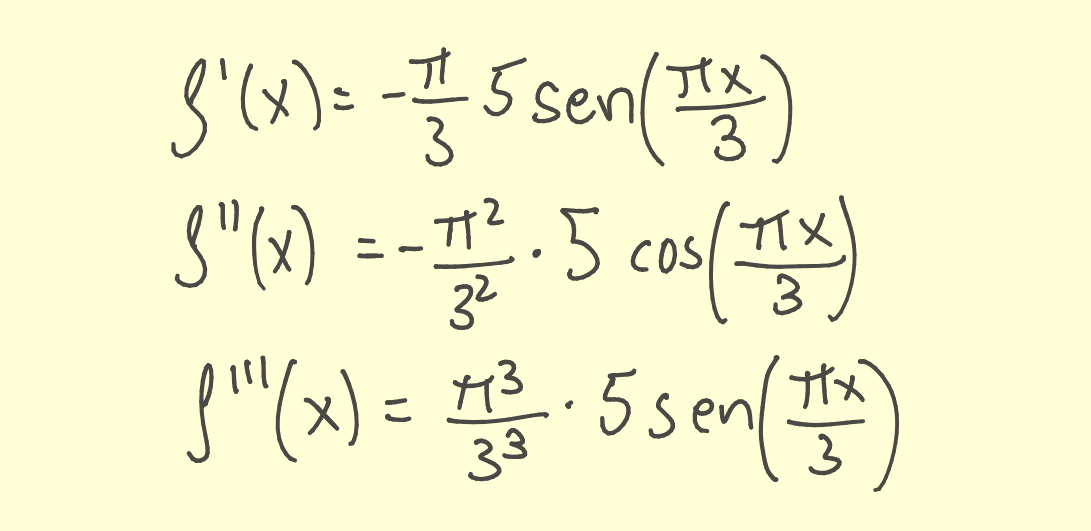
\includegraphics[width=0.5\textwidth]{src/derivadas.png}
	\caption{Derivadas de hasta orden 3 de nuestra función}
\end{figure}

Una vez teniendo la tercera derivada, se sustituye en la fórmula anterior con los demás valores de los nodos y el punto en donde estamos calculando el error:


\begin{figure}[h]
	\center
	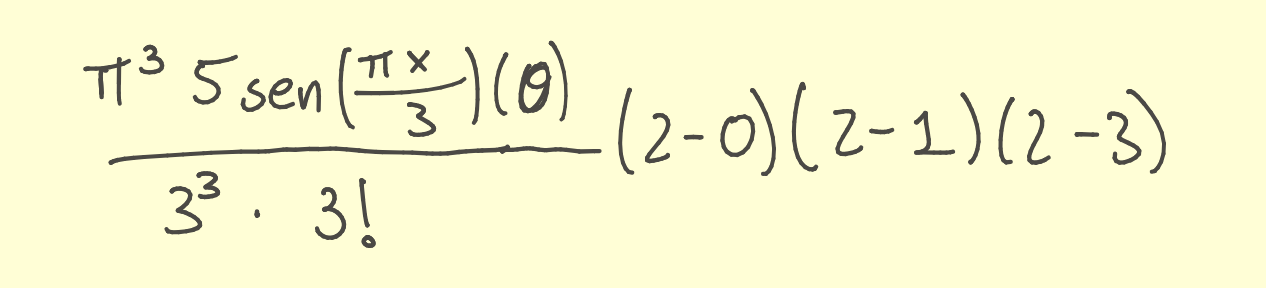
\includegraphics[width=0.5\textwidth]{src/eq2.png}
	\caption{Valores sustituidos en la fórmula}
\end{figure}

\newpage

Se desarrollará la fórmula hasta acotar el seno de nuestra función, el cual teniendo en cuenta los valores entre los que varía, podemos decir que su valor absoluto será menor o igual que 1.

\begin{figure}[h]
	\center
	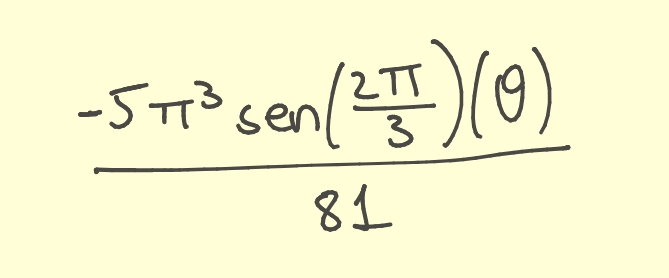
\includegraphics[width=0.5\textwidth]{src/eq3.png}
	\caption{Desarrollo de la fórmula}
\end{figure}

\begin{figure}[h]
	\center
	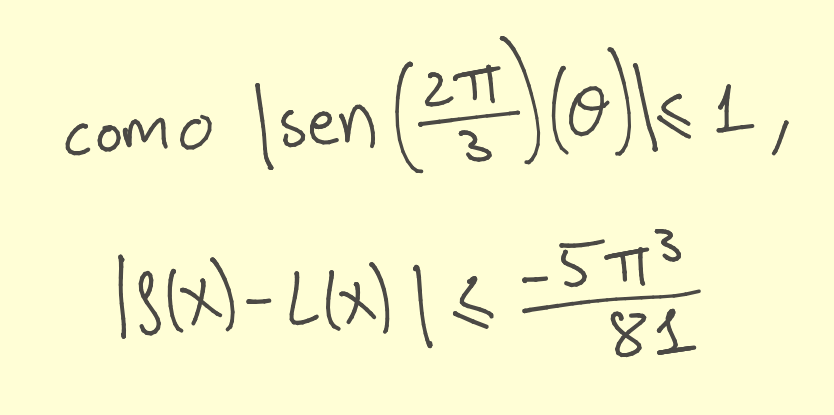
\includegraphics[width=0.5\textwidth]{src/eq4.png}
	\caption{Función de error acotada.}
\end{figure}

Por lo que finalmente, el error será


\end{document}

